\documentclass[12pt]{article}
\usepackage[top=1in, bottom=1in, right=1in, left=1in]{geometry}
\usepackage{graphicx}
\usepackage{listings}
\lstset{language=Matlab, breaklines=true}
\renewcommand*{\familydefault}{\sfdefault}

\begin{document}

\title{Financial Engineering II\\Lab Assignment 1}
\author{Kumar Harsha, 11012318}
\date{\today}
\maketitle
\tableofcontents
\newpage
\section{Question 1}
The initial option prices for various time steps are tabulated below:\\
  \begin{center}
  \begin{tabular}{c|c|c}
      Steps &Call option &Put option\\ \hline \hline
      1 &2.4634 &1.8161\\ \hline
      5 &2.1832 &1.5359\\ \hline
      10 &2.1248 &1.4775\\ \hline
      20 &2.1296 &1.4823\\ \hline
      50 &2.1272 &1.4799\\ \hline
      100 &2.1237 &1.4764\\ \hline
      200 &2.1202 &1.4729\\ \hline
      400 &2.1201 &1.4728\\ \hline
  \end{tabular}
  \end{center}

\section{Question 2}
The plots for varying time steps are as follows:\\
  \begin{center}
    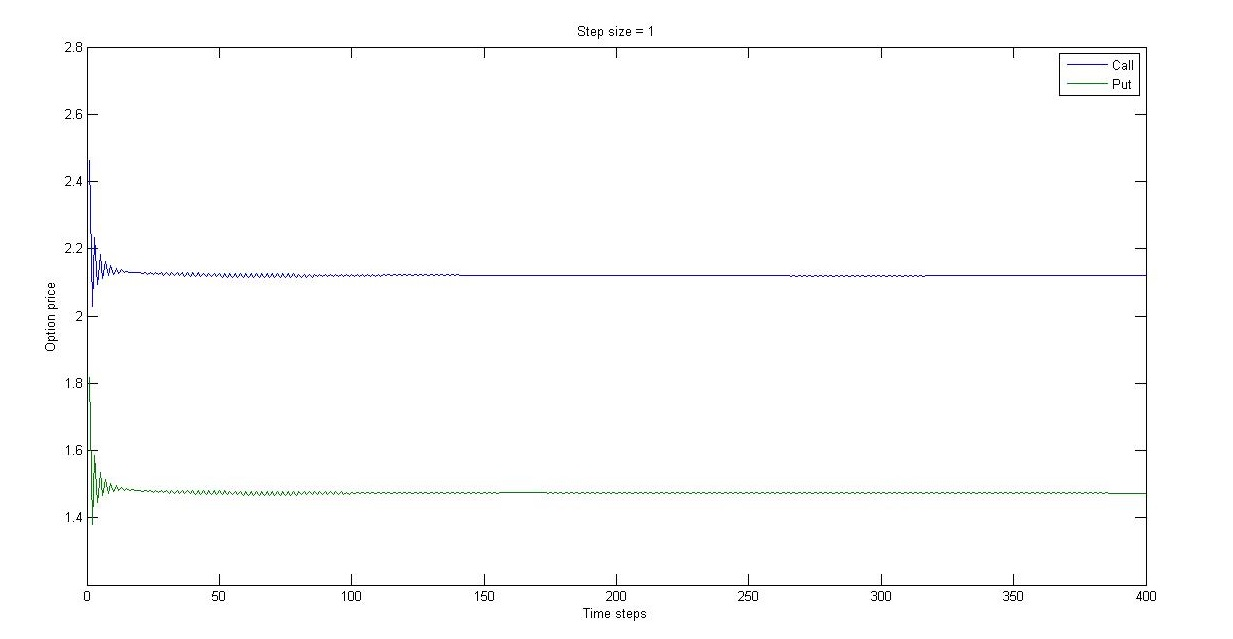
\includegraphics[width=7in]{plot1.jpg}
    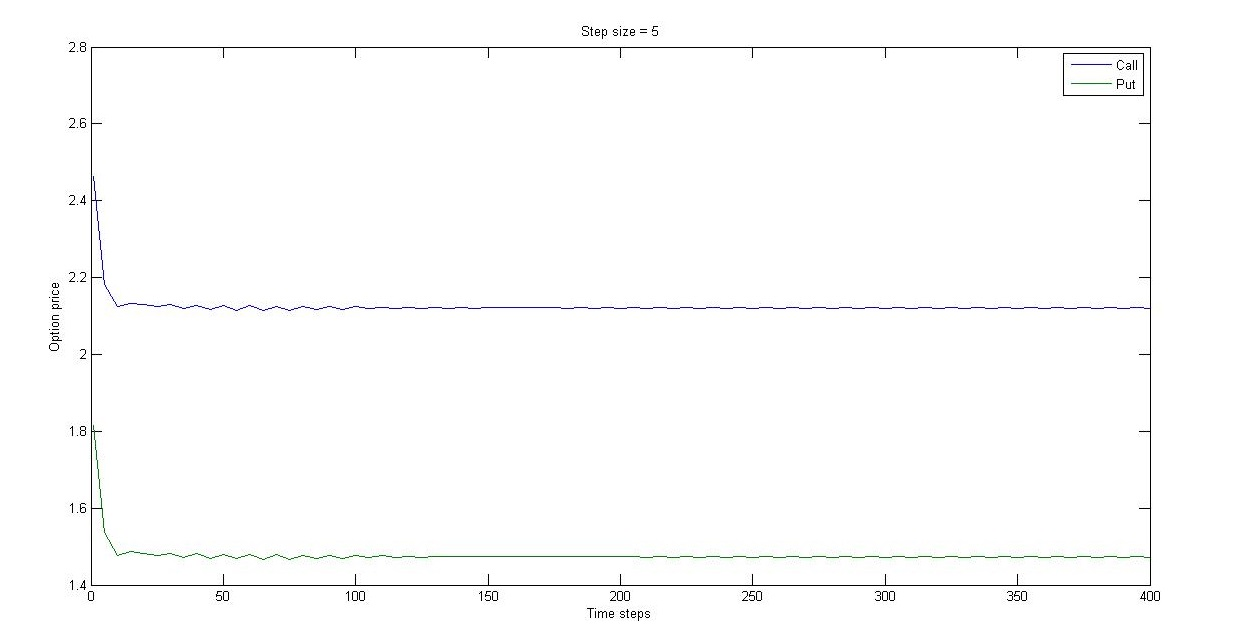
\includegraphics[width=7in]{plot2.jpg}
  \end{center}
  
  The option prices converge after the number of time steps goes beyond 100, then closely following the continuous model.

\newpage
\section{Question 3}
The values of call option at the specified time intervals are tabulated below:\\
  \begin{center}
    \begin{tabular}{ccccc}
      0 &0.30 &0.75 &1.50 &2.70\\ \hline
      2.1296	&3.7248	&7.7407	&20.2796	&66.0571\\
      0	                &1.9992	&4.6752	&14.1865	&50.3233\\
      0	                &0.9492	&2.5443	&9.3937	&37.8520\\
      0	                &0	                &1.2110	&5.7170	&27.9667\\
      0	                &0	                &0.4877	&3.0718	&20.1311\\
      0	                &0	                &0.1599	&1.3855	&13.9202\\
      0	                &0	   &0	        &0.4934	&8.9973\\
      0	                &0	   &0	                &0.1279	&5.0951\\
      0	                &0	   &0	                &0.0212	&2.1458\\
      0	                &0	   &0	                &0.0017	&0.4610\\
      0	                &0	                &0	                &0	                &0\\
      0	                &0	                &0	                &0	                &0\\
      0	                &0	                &0	                &0	                &0\\
      0	                &0	                &0	                &0	                &0\\
      0	                &0	                &0	                &0	                &0\\
      0	                &0	                &0	                &0	                &0\\
      0	                &0	                &0	                &0	                &0\\
      0	                &0	                &0	                &0	                &0\\
      0	                &0	                &0	                &0	                &0\\
      0	                &0	                &0	                &0	                &0\\
      0	                &0	                &0	                &0	                &0\\ \hline
    \end{tabular}
  \end{center}

\newpage
Following is the table for the values of the put option:
  \begin{center}
    \begin{tabular}{ccccc}
    0 &0.30 &0.75 &1.50 &2.70\\ \hline
    1.4823	&0.8236	&0.2062	&0.0005	&0\\
    0	                &1.4629	&0.5147	&0.0074	&0\\
    0	                &2.2876	&1.0582	&0.0497	    &0\\
    0	                &0	                &1.8447	&0.2057	    &0\\
    0	                &0	                &2.8017	&0.5983	    &0\\
    0	                &0	                &3.8058	&1.3200	    &0\\
    0	                &0	                &0	                &2.3365	    &0\\
    0	                &0	                &0	                &3.4839	    &0\\
    0	                &0	                &0	                &4.5764	&0.1437\\
    0	                &0	                &0	                &5.5074	&0.9106\\
    0	                &0	&0	&6.2591	&2.3929\\
    0	&0	&0	&0	&3.9333\\
    0	&0	&0	&0	&5.1542\\
    0	&0	&0	&0	&6.1220\\
    0	&0	&0	&0	&6.8891\\
    0	&0	&0	&0	&7.4972\\
    0	&0	&0	&0	&7.9792\\
    0	&0	&0	&0	&8.3612\\
    0	&0	&0	&0	&8.6640\\
    0	&0	&0	&0	&0\\
    0	&0	&0	&0	&0\\ \hline
    \end{tabular}
  \end{center}

\section{Code}
The following are the Matlab code snippets for the assignment.\\
 \subsection*{Function to evaluate option price at t=0}
   \lstinputlisting{european.m}
 \subsection*{Function to compute option price at different times}
    \lstinputlisting{dispoptionprices.m}
  \subsection*{Final code}
    \lstinputlisting{lab1.m}
\end{document}